\documentclass[a4paper,11pt]{article}

% --- Encodage et Langue ---
\usepackage[utf8]{inputenc}
\usepackage[T1]{fontenc}
\usepackage[french]{babel}

% --- Mise en page et Typographie ---
\usepackage{geometry}
\geometry{margin=2.5cm, headheight=15pt}
\usepackage{microtype}
\usepackage{lmodern}

% --- Mathématiques ---
\usepackage{amsmath, amssymb}

% --- Images ---
\usepackage{graphicx}
\usepackage{float}

% --- Couleurs et Boîtes ---
\usepackage{xcolor}
\definecolor{primary}{RGB}{0, 85, 150}      % Bleu technique
\definecolor{secondary}{RGB}{240, 248, 255} % Bleu très clair pour les fonds
\definecolor{solcolor}{RGB}{245, 250, 245}  % Vert très clair pour les solutions
\definecolor{solframe}{RGB}{60, 120, 60}    % Vert foncé pour les bordures de solution
\definecolor{termfg}{RGB}{30, 30, 30}       % Gris foncé pour le texte terminal
\definecolor{termbg}{RGB}{245, 245, 245}    % Gris très clair pour le fond terminal

\usepackage{tcolorbox}
\tcbuselibrary{skins}
\usepackage{caption} % Pour \captionof à l'intérieur des boîtes

% --- Tableaux professionnels ---
\usepackage{booktabs}
\usepackage{array}
\usepackage{multirow}

% --- Affichage de code / sortie terminal ---
\usepackage{listings}
\lstdefinestyle{termstyle}{
    basicstyle=\small\ttfamily\color{termfg},
    backgroundcolor=\color{termbg},
    frame=single,
    framerule=0.5pt,
    rulecolor=\color{gray!50},
    breaklines=true,
    columns=fullflexible,
    keepspaces=true,
    showstringspaces=false,
    numbers=none
}

% --- Titres ---
\usepackage{titlesec}
\titleformat{\section}
  {\color{primary}\Large\bfseries}
  {\thesection}{1em}{}[\titlerule]
\titleformat{\subsection}
  {\color{primary}\large\bfseries}
  {\thesubsection}{1em}{}

% --- Gestion des solutions (Mettre \solutionsfalse pour cacher les solutions) ---
\newif\ifsolutions
\solutionstrue % <--- Changez en \solutionsfalse pour la version étudiant
%\solutionsfalse % <--- Changez en \solutionsfalse pour la version étudiant

\newtcolorbox{notebox}{
  colback=secondary,
  colframe=primary,
  fonttitle=\bfseries,
  title=Notes et Conseils,
  arc=4pt,
  boxrule=0.8pt
}

\newtcolorbox{questionbox}{
  colback=secondary,
  colframe=primary,
  fonttitle=\bfseries,
  title=Questions,
  arc=4pt,
  boxrule=0.8pt
}

\newtcolorbox{solbox}{
  colback=solcolor,
  colframe=solframe,
  fonttitle=\bfseries,
  title=Solution,
  arc=4pt,
  boxrule=0.8pt
}

% --- Titre du document ---
\title{\textcolor{primary}{\Huge\bfseries TD 9 -- Électronique Numérique}\\[0.5em] \Large Conception d'un accélérateur matériel pour le calcul d'un polynôme}
\author{}
\date{}

\begin{document}

\maketitle
\vspace{-2em}

\begin{notebox}
On se propose ici de concevoir un accélérateur matériel, dédié au calcul de polynômes de rang 3. L'étude commence par une réflexion algorithmique, qui suggère des optimisations. Nous poursuivons la démarche par la manipulation abstraite de cet algorithme, à l'aide de \textit{graphes}. L'accélérateur conçu par la suite se présente comme une microarchitecture, composée classiquement d'un automate de contrôle et d'un chemin de données. On se limitera à des valeurs de $x$ entières, codées sur 32 bits.
\end{notebox}

\vspace{1em}

\section{Réflexion algorithmique}

La conception d'un accélérateur matériel naît souvent de la création d'un algorithme aux performances théoriques intéressantes (ex : compression par Transformée en Cosinus Discret), ou par la découverte d'une reformulation intéressante (ex : multiplication de Karatsuba\footnote{Nous vous invitons à vous renseigner sur ces deux curiosités mathématiques}). Nous allons ici, en miniature, suivre cette démarche.

On considère un polynôme d'ordre 3 :
\begin{equation}
P_3(x)=a_3x^3+a_2x^2+a_1x+a_0
\end{equation}

\begin{questionbox}
\begin{enumerate}
    \item \textbf{Question 1 :} Combien de multiplications et d'additions sont-elles nécessaires ?
    \item \textbf{Question 2 :} À l'aide du schéma de Hörner, normalement connu, montrer que l'on peut réduire le nombre de ces opérations.
\end{enumerate}
\end{questionbox}

\ifsolutions
\begin{solbox}
\textbf{Question 1 :} Il en faut : $3+2+1 = 6$ multiplications, et $3$ additions.

\vspace{0.5em}
\textbf{Question 2 :} On peut réécrire le polynôme précédent de la manière suivante :
\begin{align}
P_3(x) &= x(a_3x^2+a_2x+a_1)+a_0 \\
&=x(x(a_3x+a_2)+a_1)+a_0
\end{align}
On en déduit que sous cette forme, seulement \textbf{3 multiplications} sont nécessaires (en plus des 3 additions).
\end{solbox}
\fi

\section{Flot de données}

L'étude du flot de données (ou DFG : \textit{dataflow graph}) permet d'établir les dépendances du calcul. On représente généralement ces dépendances à l'aide d'un graphe orienté : chaque nœud représente une opération (ici arithmétique) ou une entrée ou une sortie. Chaque arc entre deux nœuds est étiqueté par le nom de la variable qui circule du nœud source au nœud destination. Dans notre cas, le graphe est acyclique. Il indique clairement l'enchaînement des opérations, mais il s'agit encore d'une vision abstraite du calcul, indépendante de choix d'architecture matérielle. On peut toutefois noter que ce DFG peut être vu comme une première tentative de réalisation purement combinatoire du circuit (mais son chemin critique est très certainement rédhibitoire).

\begin{questionbox}
\textbf{Question 3 :} Établir le graphe de flot de données issu du schéma de Hörner.
\end{questionbox}

\ifsolutions
\begin{solbox}
\centering
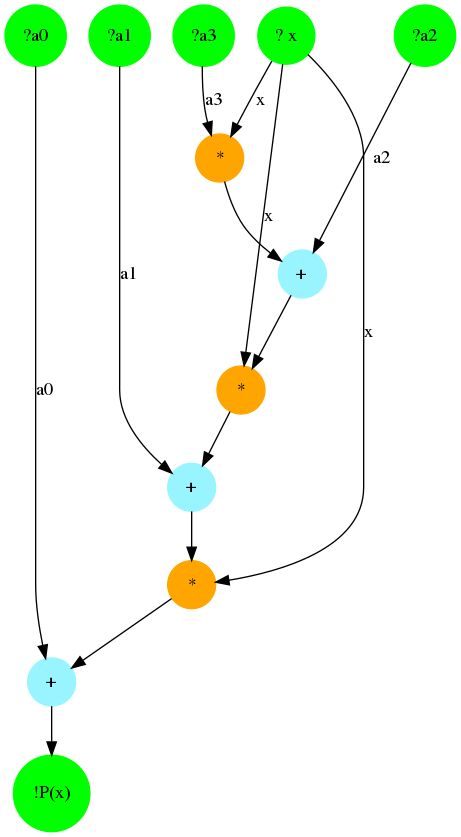
\includegraphics[scale=0.4]{./images/dfg_horner.png}
\captionof{figure}{Graphe de flot de données (DFG) du schéma de Hörner}
\end{solbox}
\fi

\section{Ordonnancement. Assignation et partage des ressources}

La notion d'\textbf{ordonnancement} permet de découper le DFG en différentes étapes de calculs, appelées \textbf{control-step} (CSTEP). Prosaïquement, cela revient à dessiner différentes lignes qui représentent effectivement cette découpe du DFG.

Chacune des étapes s'exécute en un seul cycle d'horloge. Selon la durée physique du cycle d'horloge, il est toutefois possible de réaliser des découpes du DFG plus ou moins ``longues'' : plus le cycle est long, plus il est possible d'envisager de \textbf{chaîner} un ensemble d'opérations. À la fin du cycle, on devra veiller à échantillonner les données produites : formulé autrement, on peut dire que la découpe en CSTEPs détermine où devront se trouver les \textit{registres intermédiaires} de calcul.

En général, les opérateurs de calculs et les registres de calcul représentent la majeure partie de la surface occupée sur silicium. Il est souvent souhaitable de les utiliser avec parcimonie et notamment de les partager dès que cela est possible. On réalise l'\textbf{assignation} des opérations aux opérateurs afin d'établir où se réaliseront effectivement les calculs du DFG abstrait. Bien évidemment, à la fin d'un CSTEP tous les opérateurs utilisés sont à nouveau disponibles pour le CSTEP suivant, ce qui donne des opportunités de partage de ressources entre opérations ordonnancées sur deux CSTEPs différents. Ces informations d'assignation peuvent être également annotées sur le DFG : à côté de l'opération abstraite du DFG, on peut indiquer sur quel opérateur matériel elle s'exécutera.

Avant même la phase d'assignation, le concepteur se donne par ailleurs un objectif en terme de nombre de ressources utilisées au total : c'est la phase d'\textbf{allocation de ressources}. Il peut se donner le droit d'utiliser tel nombre de multiplieurs, tel nombre d'additionneurs, tel nombre de registres, etc. Parmi les contraintes, on retrouve d'autres paramètres variés et en particulier la fréquence attendue du circuit. On se fixe ici une fréquence d'horloge de 100 MHz.

\begin{questionbox}
\begin{enumerate}
    \item \textbf{Question 4 :} On s'alloue 1 multiplieur et un additionneur. Le multiplieur a un temps de calcul de 7 ns et l'additionneur de 2 ns. Concernant les registres, on considère que leur temps de setup et hold sont très inférieurs, et non significatifs par rapport aux opérateurs. Proposer un ordonnancement qui vous semble judicieux. À combien de CSTEPs aboutissons-nous ?
    \item \textbf{Question 5 :} Réaliser l'assignation des ressources et notamment des registres.
\end{enumerate}
\end{questionbox}

\ifsolutions
\begin{solbox}
\textbf{Question 4 :} On voit sur le DFG que le calcul de multiplication et d'addition se suivent. Le chemin critique de cet enchaînement est de $7+2=9$ ns. Or, la fréquence de fonctionnement des registres est de 100 MHz soit un temps de cycle de 10 ns : ce budget de 10 ns laisse parfaitement le temps aux signaux de traverser à la fois le multiplieur et l'additionneur, dans un même cycle d'horloge. Cela est d'autant plus vrai que les temps de setup et hold sont considérés comme négligeables dans l'énoncé. On peut donc chaîner les opérateurs matériels dans le même cycle. Par contre, à la fin de cette portion (répétée) de circuit, il faudra échantillonner les signaux, dans des bascules D (registres). Le schéma suivant donne 3 CSTEPs. On suppose que les entrées et sorties sont également ``clockées'' (échantillonnées), ce qui est une bonne pratique.

\vspace{0.5em}
\centering
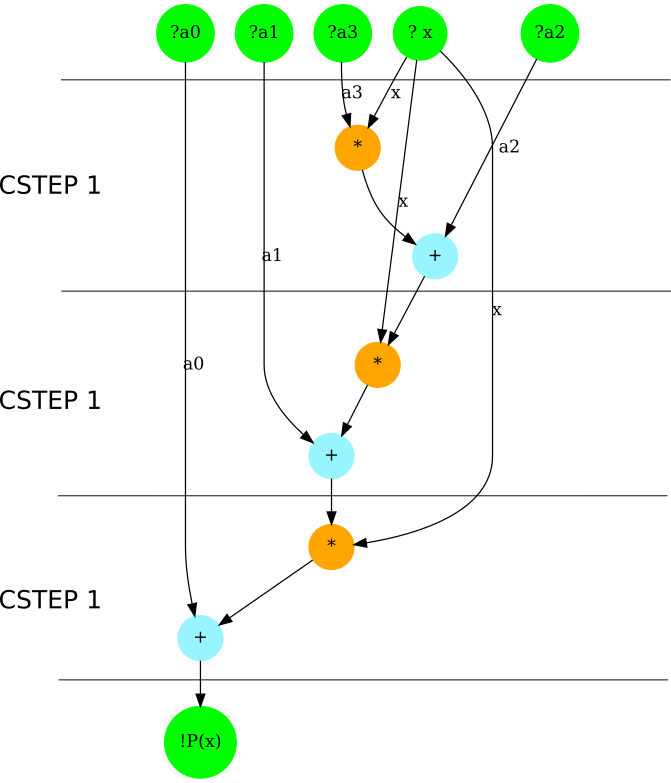
\includegraphics[scale=0.5]{./images/dfg_horner_sched.png}
\captionof{figure}{DFG ordonnancé en 3 CSTEPs}

\end{solbox}
\fi

\ifsolutions
\begin{solbox}
\textbf{Question 5 :} On annote les ressources sur le schéma : il s'agit désormais d'opérateurs matériels et non plus d'opérations abstraites. Ces opérateurs peuvent être réutilisés à chaque cycle (CSTEP). De même un registre dont on n'a plus besoin peut être réutilisé. C'est le cas du registre R3, qui contient initialement le premier coefficient lu. Après cette lecture, on peut utiliser R3 pour les calculs des variables temporaires (intermédiaires) de calcul.

\vspace{0.5em}
\centering
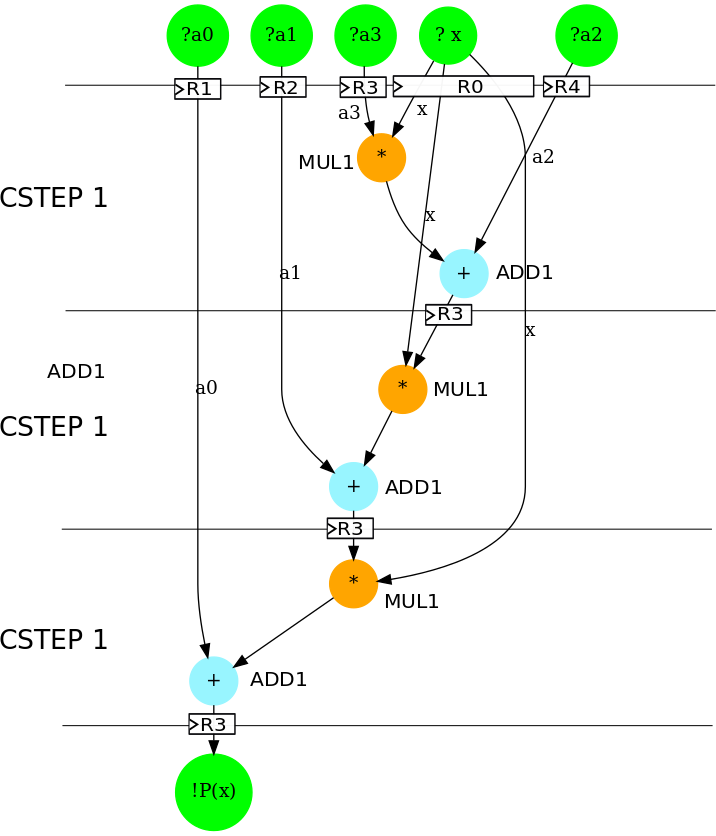
\includegraphics[scale=0.4]{./images/dfg_horner_binding.png}
\captionof{figure}{DFG avec assignation des ressources}
\end{solbox}
\fi

%%\newpage

\section{Microarchitecture : automate de contrôle et datapath}

Dès lors qu'un ordonnancement est choisi, il est alors aisé de décrire un automate et un chemin de donnée. L'automate permet de séquencer les différentes étapes. Il réalise en outre, pour chacune d'entre elles, les actions appropriées. À l'issue de l'assignation, ces actions reviennent à contrôler les multiplexeurs d'un chemin de données (datapath) : ces multiplexeurs servent soit à échantillonner une donnée à l'entrée d'un registre, soit à router une donnée vers un opérateur matériel.

\begin{questionbox}
\begin{enumerate}
    \item \textbf{Question 6 :} Dessiner l'automate de contrôle.
    \item \textbf{Question 7 :} Dessiner un chemin de données.
    \item \textbf{Question 8 :} Compléter l'automate pour indiquer les actions réalisées dans chaque état.
\end{enumerate}
\end{questionbox}

\ifsolutions
\begin{solbox}
\textbf{Question 6 :}

\vspace{0.5em}
\centering
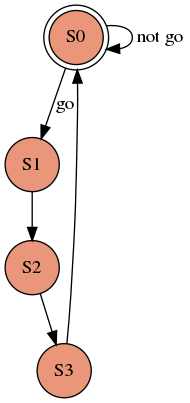
\includegraphics[scale=0.4]{./images/fsm.png}
\captionof{figure}{Automate de contrôle}
\end{solbox}
\fi

\ifsolutions
\begin{solbox}
\textbf{Question 7 :} Pour déterminer le chemin de données (datapath), on observe le DFG ordonnancé et alloué (question 5). Il s'agit essentiellement de déterminer les opérandes des opérateurs. Prenons le Multiplieur MUL1 : on voit que ses opérandes sont R0 et R3 lors du CSTEP 1, et à nouveau R0 et R3 aux CSTEPs 2 et 3. Le chemin entre les registres et l'entrée de MUL1 est donc très simple et direct. Observons maintenant ADD1 :
\begin{itemize}
    \item dans le CSTEP 1, ADD1 opère sur le résultat combinatoire de MUL1 et sur R4
    \item dans le CSTEP 2, ADD1 opère sur le résultat combinatoire de MUL1 et sur R2
    \item dans le CSTEP 3, ADD1 opère sur le résultat combinatoire de MUL1 et sur R1
\end{itemize}
On peut en déduire que pour assurer ces 3 fonctionnements, il est nécessaire d'adjoindre un multiplexeur sur le second opérande de ADD1, dont les sources sont R4, R2 et R1.

Notons que nos deux opérateurs sont commutatifs, ce qui a grandement simplifié notre analyse. On en déduit une version, encore incomplète, du datapath, présentée sur la figure suivante.

\vspace{0.5em}
\centering
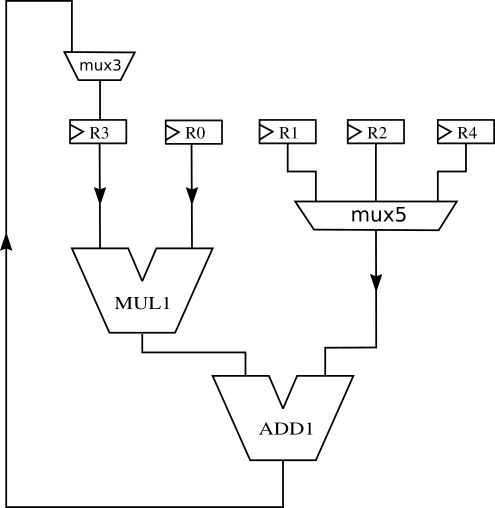
\includegraphics[scale=0.4]{./images/datapath_primitif.png}
\captionof{figure}{Datapath primitif (incomplet)}
\end{solbox}
\fi

\ifsolutions
\begin{solbox}
\paragraph{Suite}

Quelques détails restent à régler : comment sont acheminés les entrées et calculs intermédiaires, vers ces registres ? Il faut bien penser à l'échantillonnage des entrées et leur stockage tout au long du calcul. Là encore on repose sur un multiplexeur, dont la commande peut jouer ce rôle. Afin de ne pas modifier la donnée stockée (potentiellement ré-échantillonnée à chaque cycle), on fait ainsi ``recirculer'' la donnée de la sortie Q à l'entrée D des bascules.

Désormais notre datapath est complet. Reste à déterminer les instants de contrôles des multiplexeurs, émis par le contrôleur (FSM).

\vspace{0.5em}
\centering
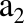
\includegraphics[scale=0.4]{./images/datapath.png}
\captionof{figure}{Datapath complet}

\vspace{0.5em}
On numérote les entrées des multiplexeurs : ces valeurs correspondront aux valeurs du signal de commande qu'il faudra envoyer au multiplexeur pour qu'il fasse passer l'entrée correspondante sur sa sortie. Cela nous permettra de piloter le cheminement des données (question suivante).

\vspace{0.5em}
\centering
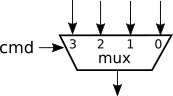
\includegraphics[scale=0.6]{./images/mux.png}
\captionof{figure}{Numérotation des entrées des multiplexeurs}
\end{solbox}
\fi

\ifsolutions
\begin{solbox}
\textbf{Question 8 :} On se propose de présenter cet automate sous la forme tabulée suivante. Ce tableau fait apparaître les \textit{transferts de registres}, ainsi que les micro-actions correspondantes, sur les multiplexeurs.

\vspace{0.5em}
\centering
\renewcommand{\arraystretch}{1.2}
\begin{tabular}{|c|c|c|c|}
\toprule
\textbf{État} & \textbf{Effet algorithmique} & \textbf{Transferts de registres} & \textbf{Contrôle Mux} \\
\midrule
\multirow{6}{*}{S0} & \multirow{6}{*}{Arrivée des données} & $R0 \leftarrow x$ & $cmd_0 \leftarrow 1$ \\
 & & $R1 \leftarrow a_0$ & $cmd_1 \leftarrow 1$ \\
 & & $R2 \leftarrow a_1$ & $cmd_2 \leftarrow 1$ \\
 & & $R3 \leftarrow a_3$ & $cmd_3 \leftarrow 1$ \\
 & & $R4 \leftarrow a_2$ & $cmd_4 \leftarrow 1$ \\
 & & & $cmd_5 \leftarrow 0$ \\
\midrule
\multirow{6}{*}{S1} & \multirow{6}{*}{$t_1=a_3 \times x+a_2$} & & $cmd_0 \leftarrow 0$ \\
 & & & $cmd_1 \leftarrow 0$ \\
 & & & $cmd_2 \leftarrow 0$ \\
 & & $R3 \leftarrow (R3 \times R0)+R4$ & $cmd_3 \leftarrow 2$ \\
 & & & $cmd_4 \leftarrow 0$ \\
 & & & $cmd_5 \leftarrow 0$ \\
\midrule
\multirow{6}{*}{S2} & \multirow{6}{*}{$t_2=t_1 \times x+a_1$} & & $cmd_0 \leftarrow 0$ \\
 & & & $cmd_1 \leftarrow 0$ \\
 & & $R3 \leftarrow (R3 \times R0)+R2$ & $cmd_2 \leftarrow 0$ \\
 & & & $cmd_3 \leftarrow 2$ \\
 & & & $cmd_4 \leftarrow 0$ \\
 & & & $cmd_5 \leftarrow 1$ \\
\midrule
\multirow{6}{*}{S3} & \multirow{6}{*}{$P(x)=t_2 \times x+a_0$} & & $cmd_0 \leftarrow 0$ \\
 & & & $cmd_1 \leftarrow 0$ \\
 & & $R3 \leftarrow (R3 \times R0)+R1$ & $cmd_2 \leftarrow 0$ \\
 & & & $cmd_3 \leftarrow 2$ \\
 & & & $cmd_4 \leftarrow 0$ \\
 & & & $cmd_5 \leftarrow 2$ \\
\bottomrule
\end{tabular}

\vspace{1em}
Quelques remarques :
\begin{itemize}
    \item On notera au passage que ces transferts de registres ressemblent à ce que réalise un langage de programmation de bas niveau : l'assembleur. Toutefois, nos transferts de registres sont ici plus puissants que l'assembleur : plusieurs transferts peuvent avoir lieu en même temps, en parallèle, alors qu'en assembleur traditionnel chaque transfert se fait séquentiellement.
    \item L'opération de multiplication suivie d'une addition est si fréquente dans le domaine scientifique, qu'il existe un opérateur dédié : le \textbf{MULACC}. Il est présent notamment dans les processeurs de traitement du signal, appelés DSP (\textit{digital signal processors}, les plus connus étant ceux de Texas Instruments). Les FPGA modernes possèdent en plus de leur matrice de LUTs, un ensemble de tels opérateurs optimisés.
\end{itemize}
\end{solbox}
\fi


%\newpage

\section{Dimensionnement des registres}

Une difficulté récurrente lorsqu'on traduit un algorithme en microarchitecture réside dans le dimensionnement des signaux, c'est-à-dire la détermination du nombre de bits nécessaires à la représentation des nombres, sans perte d'information préjudiciable. On parle aussi de leur \textit{dynamique}. Il y a perte d'information lors d'une troncature (élimination brutale de bits à un certain rang).

\begin{questionbox}
\begin{enumerate}
    \item \textbf{Question 9 :} Soient deux signaux $s_n$ et $s_{n'}$ entiers codés respectivement sur $n$ et $n'$ bits. Déterminer le nombre de bits nécessaires à l'addition $s_n+s_{n'}$, sans perte d'information.
    \item \textbf{Question 10 :} Même question pour $s_n \times s_{n'}$.
    \item \textbf{Question 11 :} En déduire la dynamique des signaux apparaissant dans le datapath.
\end{enumerate}
\end{questionbox}

\ifsolutions
\begin{solbox}
\textbf{Question 9 :} Par exemple, avec $n=8$ et $n'=8$, $s_n, s_{n'} \in \{0 \dots 255\}$ et $s_n+s_{n'} \in \{0 \dots 510\}$. On se convainc facilement que le nombre de bits pour le résultat de l'addition est $\mathbf{max(n,n')+1}$.

\vspace{0.5em}
\textbf{Question 10 :} Pour la multiplication le résultat est $\mathbf{n+n'}$.

\vspace{0.5em}
\textbf{Question 11 :} À la fin de chaque CSTEP, la dynamique des signaux calculés augmente. Si chaque entrée est codée sur un même nombre $n$ de bits :
\begin{itemize}
    \item CSTEP 1 : R3 nécessite $2n+1$ bits
    \item CSTEP 2 : R3 nécessite $(2n+1)+n+1=3n+2$ bits
    \item CSTEP 3 : R3 nécessite $(3n+2)+n+1=4n+3$ bits
\end{itemize}
À titre d'exemple, partant de $n=8$ bits, on obtient \textbf{35 bits} nécessaires en sortie.
\end{solbox}
\fi

%\newpage

\section{Codage VHDL}

Le code VHDL de cet accélérateur est fourni sur Moodle, ainsi qu'un banc de test. La syntaxe de VHDL est complexe et nouvelle pour vous, mais vous êtes à même d'en comprendre les grandes lignes.

\begin{questionbox}
\begin{enumerate}
    \item \textbf{Question 12 :} Observez attentivement le code de l'accélérateur. Dessiner l'architecture générale du système. Discutez avec votre encadrant afin de bien vérifier que vous avez compris la correspondance avec vos schémas précédents.
    \item \textbf{Question 13 :} Observez attentivement le code du banc de test. Discutez avec votre encadrant afin de bien vérifier que vous avez compris son fonctionnement.
    \item \textbf{Question 14 :} La simulation ne sera pas réalisée en séance, mais une vidéo sera mise à disposition.
\end{enumerate}
\end{questionbox}

\ifsolutions
\begin{solbox}
\textbf{Question 12 :}


\centering
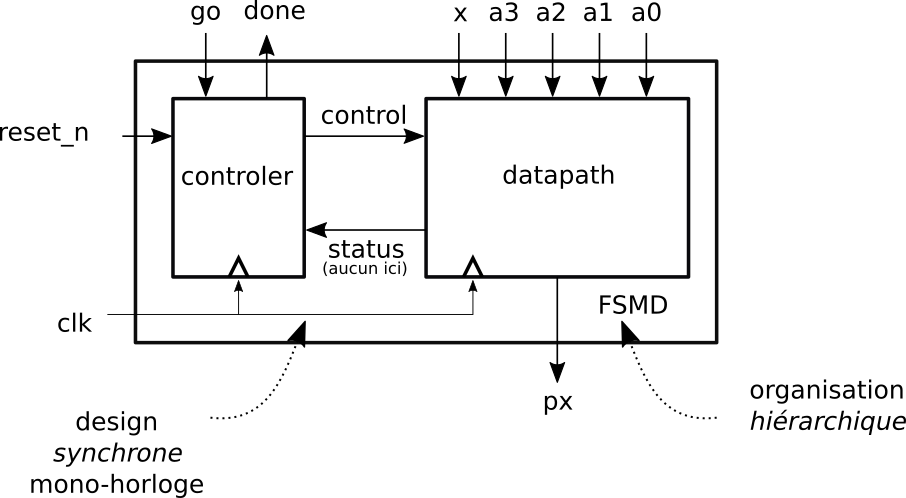
\includegraphics[scale=0.4]{./images/fsmd.png}
\captionof{figure}{Architecture générale du système (FSMD)}
\end{solbox}
\fi

\ifsolutions
\begin{solbox}

\textbf{Question 13 :} Le banc de test se présente comme un design classique : il est composé d'une entité et d'une architecture. Toutefois l'entité ne possède aucun port d'entrée-sortie. Cela est parfaitement normal, car notre testbench représente une ``expérience virtuelle'', dans un laboratoire tout aussi virtuel, entièrement équipé et autonome ! Il n'a besoin d'aucune information extérieure. L'architecture représente la paillasse où l'on prépare un ``setup expérimental'' : au centre, on retrouve bien entendu le circuit à tester, et tout autour de lui des instruments virtuels, sous forme de processus qui fonctionnent en parallèle, les uns des autres : générateurs de signaux, sondes, outils de diagnostique etc.

Notre testbench réalise également une comparaison des signaux issus de notre circuit (\texttt{done} et \texttt{px}) avec un modèle de référence. Ce modèle de référence est ici calculé également par VHDL. Dans notre cas, VHDL est en effet capable de calculer un polynôme, de manière ``informatique''. Il aurait été assez maladroit de recourir à un modèle de référence Python ou Matlab pour écrire une référence si simple. Toutefois, cela arrive fréquemment que les équipes en présence n'aient pas la même culture. Les algorithmiciens, qui fournissent de tels modèles de références, connaissent rarement VHDL.


\centering
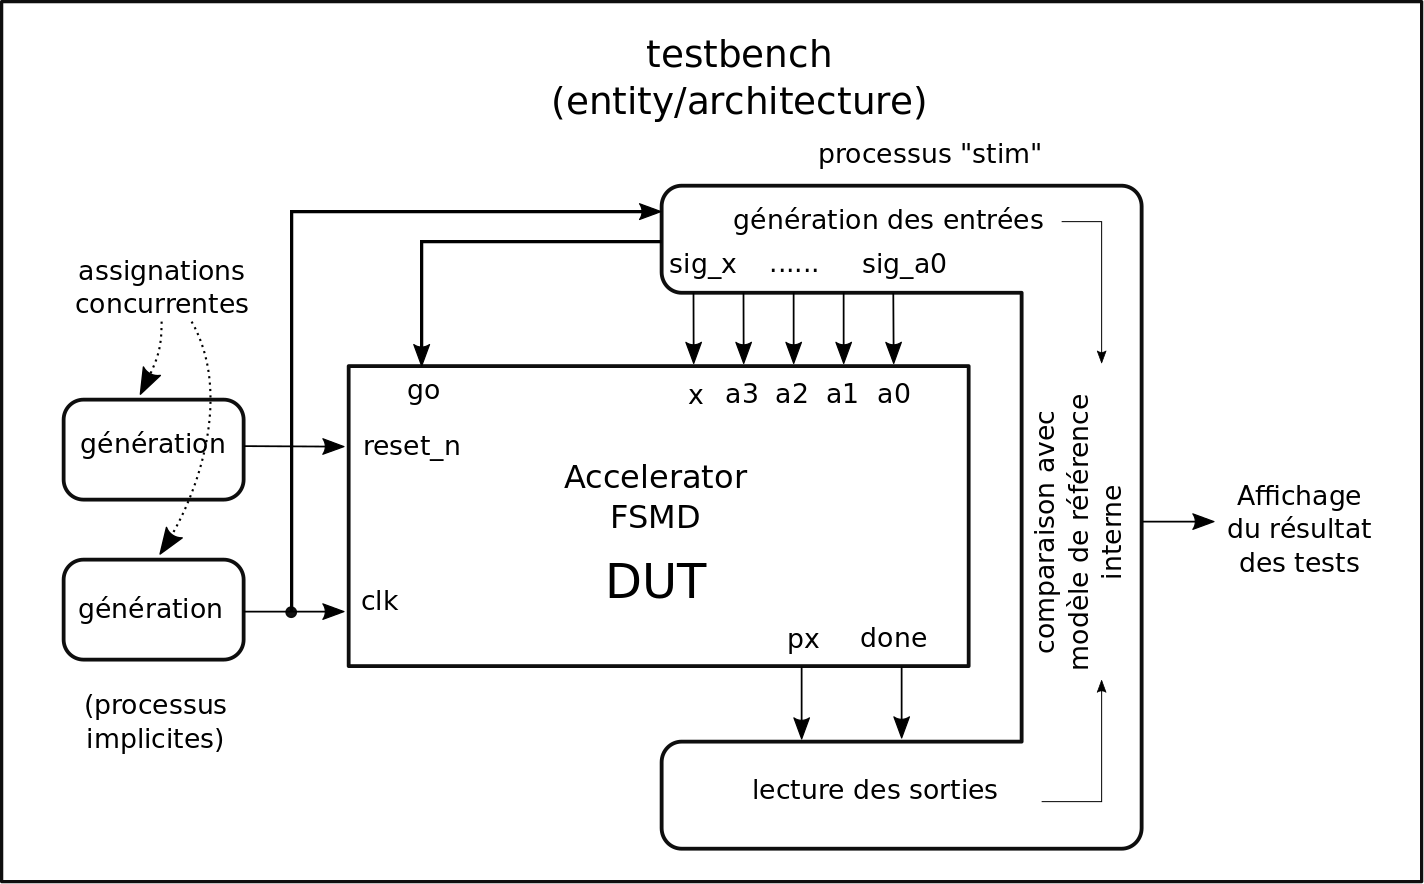
\includegraphics[scale=0.3]{./images/fsmd_tb.png}
\captionof{figure}{Architecture du banc de test}
\end{solbox}
\fi

\ifsolutions
\begin{solbox}
\textbf{Question 14 :} La simulation se fait ici sous Linux, à l'aide de GHDL. GHDL permet de générer un simulateur compilé. Cette génération se fait en 3 grandes étapes :
\begin{itemize}
    \item \textbf{Analyse} des fichiers avec l'option \texttt{-a} de ghdl.
    \item \textbf{Élaboration} du simulateur avec l'option \texttt{-e} de ghdl.
    \item \textbf{Lancement} (\textbf{run}) du simulateur avec l'option \texttt{-r} de ghdl.
    \item \textbf{Visualisation} des résultats de simulation avec GtkWave.
\end{itemize}

Ces commandes répétitives sont facilement automatisables sous Linux. Un script bash \texttt{compile.x} est fourni sur Moodle.


On obtient le \textbf{chronogramme} suivant :


\centering
\includegraphics[scale=0.3]{./images/gtkwave_commente.png}
\captionof{figure}{Chronogramme de simulation commenté}
\end{solbox}
\fi

\ifsolutions
\begin{solbox}

Dans le terminal Linux apparaissent les messages du simulateur, ainsi que les ``reports'' que l'on a décrits en VHDL :


\begin{lstlisting}[style=termstyle]
~/JCLL/ens/UE1.2-Electronique/TD/9_BE_Horner/VHDL$ ./compile.x
============ cleaning  ============
======= analyzing vhdl files ======
=> controler_pkg.vhd
=> controler.vhd
=> datapath.vhd
=> fsmd.vhd
=> fsmd_tb.vhd
======= elaborating simulation ======
=> fsmd_tb
========= running simulation ========
@0ms   :(report note): running testbench for fsmd(rtl)
@0ms   :(report note): waiting for asynchronous reset
@215ns :(report note): p(x)=4x^3 +3x^2 + 2x + 1
@215ns :(report note): sending parameters a0...a3
@315ns :(report note): expected p(0)=1
@365ns :(report note): actual : p(0)=1
@365ns :(report note): expected p(1)=10
@415ns :(report note): actual : p(1)=10
@415ns :(report note): expected p(2)=49
@465ns :(report note): actual : p(2)=49
@465ns :(report note): expected p(3)=142
@515ns :(report note): actual : p(3)=142
@515ns :(report note): expected p(4)=313
@565ns :(report note): actual : p(4)=313
@565ns :(report note): expected p(5)=586
@615ns :(report note): actual : p(5)=586
@615ns :(report note): expected p(6)=985
@665ns :(report note): actual : p(6)=985
@665ns :(report note): expected p(7)=1534
@715ns :(report note): actual : p(7)=1534
@715ns :(report note): expected p(8)=2257
@765ns :(report note): actual : p(8)=2257
@765ns :(report note): expected p(9)=3178
@815ns :(report note): actual : p(9)=3178
@815ns :(report note): expected p(10)=4321
@865ns :(report note): actual : p(10)=4321
@865ns :(report note): expected p(11)=5710
@915ns :(report note): actual : p(11)=5710
@915ns :(report note): expected p(12)=7369
@965ns :(report note): actual : p(12)=7369
@965ns :(report note): expected p(13)=9322
@1015ns:(report note): actual : p(13)=9322
@1015ns:(report note): expected p(14)=11593
@1065ns:(report note): actual : p(14)=11593
@1065ns:(report note): expected p(15)=14206
@1115ns:(report note): actual : p(15)=14206
@1115ns:(report note): expected p(16)=17185
@1165ns:(report note): actual : p(16)=17185
@1165ns:(report note): expected p(17)=20554
@1215ns:(report note): actual : p(17)=20554
@1215ns:(report note): expected p(18)=24337
@1265ns:(report note): actual : p(18)=24337
@1265ns:(report note): expected p(19)=28558
@1315ns:(report note): actual : p(19)=28558
@1315ns:(report note): end of simulation
@1315ns:(report note): number of errors : 0 / 20 tests
============== viewing ==============
GTKWave Analyzer v3.3.86 (w)1999-2017 BSI
[0] start time.
[1515000000] end time.
\end{lstlisting}
\end{solbox}
\fi

\end{document}
